\section{Zielsetzung}
\label{sec:Zielsetzung}
In diesem Versuch wird die Emission von Elektronen aus einer Metalloberfläche untersucht. Dazu wird eine Kennlinie einer Hochvakuumdiode erstellt und daraus Austrittsarbeit bestimmt und Temperaturabhängigkeit analysiert.


\section{Theorie}
\label{sec:Theorie}
Auf dem Kristallgitter von Metallen sitzen Leitungselektronen, welche sich im Potential der Ionen befinden. Um aus dem Metallinneren zu entkommen, müssen die Elektronen gegen das Potential anlaufen. Dabei bringen sie ein Austrittsarbeit auf.
Da die Elektronen dem Pauli-Verbot unterliegen, und sie somit alle unterschiedliche Energien besitzen müssen, haben sie am absoluten Nullpunkt noch eine endliche Energie. Diese ist Abhängig von der Anzahl der Elektronen $n$, und wird auch als Fermische Grenzenergie $\zeta$ bezeichnet.
Die Fermi-Diracsche Verteilungs-Funktion
\begin{align}
f(E) = \frac{1}{\exp(\frac{E-\zeta}{kT})+1}
\end{align}
beschreibt die Wahrscheinlichkeit dafür, dass ein Zustand mit einer gewissen Energie $E$ besetzt ist.
Die Kurve dieser Funktion ist in Abbildung (1) dargestellt.
Bei Elektronen, welche das Material verlassen können, kann mit der Näherung
\begin{align}
f(E) = \exp(\frac{E-\zeta}{kT})
\end{align}
gerechnet werden.
\begin{figure}[H]
  \centering
  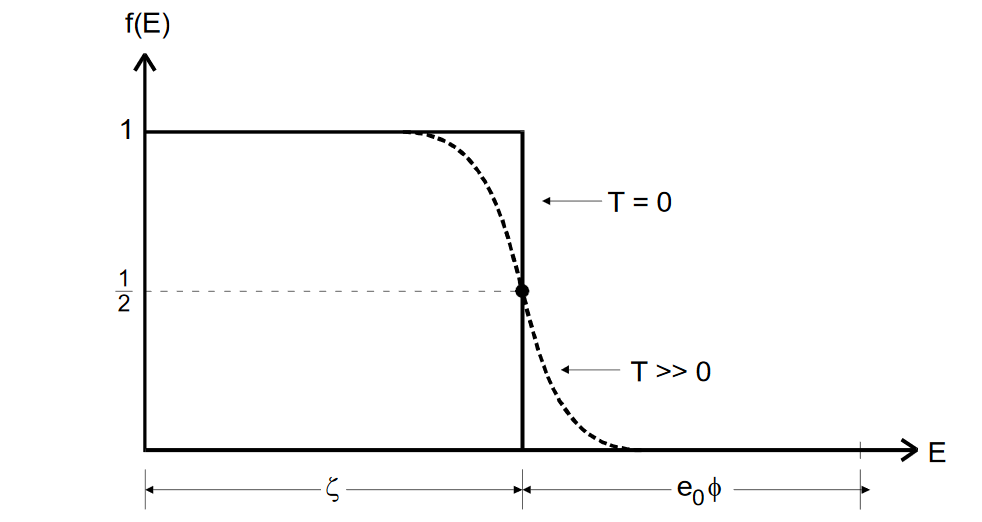
\includegraphics[width=0.8\textwidth]{fermi.png}
  \caption{Kurve der Fermi-Dirac Verteilung\cite{kent}.}
  \label{fig:aufbau}
\end{figure}

Um den Zusammenhang zwischen Anodenstrom $I_A$ und Potential zu erkennen, dient eine Kennlinie einer Hochvakuumdiode. Ein Verlauf ist in Abbildung (2) dargestellt.
\begin{figure}[H]
  \centering
  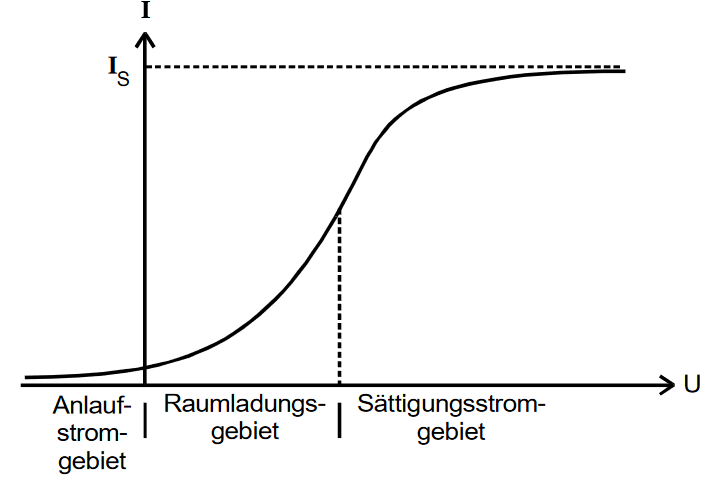
\includegraphics[width=0.7\textwidth]{k.png}
  \caption{Verlauf einer Kennlinie \cite{kent}.}
  \label{fig:aufbau}
\end{figure}
Die Kurve lässt sich in drei Bereiche einteilen: Das Anlaufstrom-, Raumladungs-, und Sättigungsstromgebiet. Das Anlaufstromgebiet liegt dort, wo das Potential negativ ist.
Dass die Stromdichte bei $V=0$ nicht Null ist, liegt daran, dass die Elektronen eine Eigengeschwindigkeit besitzen, wenn sie aus der Kathode austreten. Die Elektronen mit Energieüberschuss $\Delta E = E - ( \zeta + e_0 \phi)$ können gegen ein Gegenfeld anlaufen und die Energie ist größer als die Austrittsarbeit.
Das Anodenmaterial besitzt eine größere Austrittsarbeit $\phi_A$. Bei angelegtem äußerden Potential $V$ zwischen Anode und Kathode, verschieben sich die Fermi-Oberflächen um $e_0V$ gemäß Abbildung (3).
\begin{figure}[H]
  \centering
  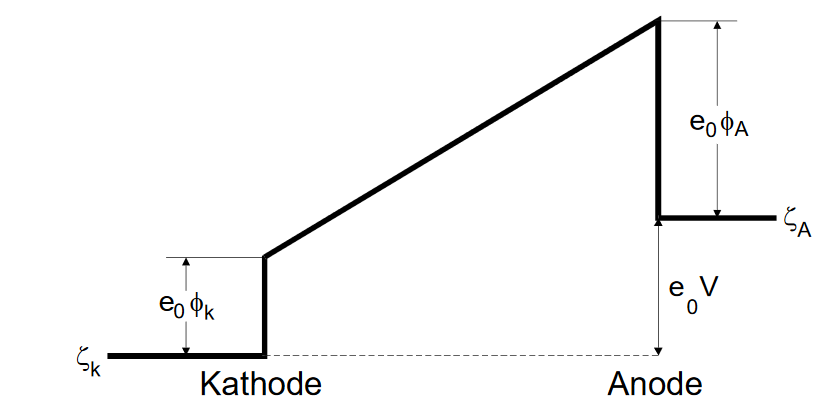
\includegraphics[width=0.8\textwidth]{blah.png}
  \caption{Verschiebung der Potentiale von Kathode und Anode \cite{kent}.}
  \label{fig:aufbau}
\end{figure}
Die Elektronen, welche die Anode erreichen, müssen eine um $e_0 \phi_A + e_0 V$ höhere Energie besitzen. Ein Zusammenhang zwischen Strom und Potential gibt folgende Gleichung
\begin{align}
j(V) = j_0 \exp(-\frac{e_0 \phi_A + e_0 V}{k T}) = const \exp(-\frac{e_0 V}{k T})
\end{align}
Das Raumladungsgebiet schließt an das Anlaufgebiet an. Bei niedriger Spannung erreichen nur wenige Elektronen die Anode. Das Ohmsche Gesetz ist bei einer Diode nicht gültig, da die Elektronen keine konstante Geschwindigkeit in Richtung Anode besitzen. Die Raumladungsdichte $\rho$ ist also eine vom Ort abhängige Funktion, und nimmt in Richtung Anode ab, da die Stromdichte durch die Kontinuitätsgleichung
\begin{align}
j = -\rho v
\end{align}
beschrieben ist.
Die Raumladungsdichte schirmt das elektrische Feld von der Kathode ab, weshalb nicht alle Elektronen das Anodenfeld erreichen. Das Gebiet kann durch die Gleichung
\begin{align}
j = \frac{4}{9} \epsilon_0 \sqrt{2 e_0/m_0}\frac{V^\frac{3}{2}}{a^2}
\end{align}
beschrieben werden und heißt Langmuir-Schottkysches Raumladungsgesetz. Die Größe $a$ beschreibt den Abstand der Kathode und der Anode.
An dieses Gebiet schließt das Sättigungsstromgebiet an. Die Raumladungsgleichung ist nicht für alle Spannungen gültig; der Anodenstrom nähert sich einem Sättigungswert an. Dieser ist durch die Richardson-Gleichung
\begin{align}
j_S(T) = 4 \pi \frac{e_0 m_0 k^2}{h^3}T^2 \exp(\frac{-e_0 \phi}{k T})
\end{align}
gegeben. Die Sättigungsstromdichte $j_S$ gibt anschaulich die Zahl der Elektronen an, die pro Zeit und Flächeneinheit emittiert werden. Außerdem ist sie Temperaturabhängig. In diesem Gebiet ist die Spannung so hoch, dass alle Elektronen die Anode erreicht haben.

